\chapter{Kernel CN:\ Static semantics}%

\margintoc{}

I have covered a large amount of background to the type system so far:
\intro{Core}, liquid types, bidirectional type systems, linear types, precise
separation logic assertions, monadic syntax for the latter and its relation to
kernel syntax for types, let-normalisation and explicit resource terms in
\kl{ResCore}. I use all of these ingredients in defining the type system for
\kl{kernel CN} that I will explain in this chapter. Some of the sections will
based on my contributions to~\sidetextcite{pulte2023cn}%

The \kl{Kernel CN} type system is ordinary \kl{CN}, defined over \kl{ResCore}
instead of \kl{Core}, without any type or resource inference. In particular, It
requires that that all universal quantifiers are explicitly instantiated, that
all existential quantifiers have explicit witnesses, and all resource
operations are embedded into the program itself as linearly typed proof terms.
It does not require proof terms for the logical properties, since by
construction all of the entailments fall into the decidable SMT fragment; many
rules rely on this. The lack of inference make it a simpler language for which
to prove type soundness, whilst still demonstrating all the key ingredients
mentioned above. Since it handles the majority of C, the entire system is very
large, and so I will only discuss the main features.

There are some additional minor differences between the implementation and the
formalisation. As I mentioned \nameref{sec:desugaring}, the formalisation has a
richer grammar of resources: this makes defining predicates to represent tagged
unions more succinct, and allows for opening predicates in more cases. The
formalisation assumes that iterated resources output arguments have type array
of records, whereas the implementation uses records of arrays.\sidenote{This
purely a notational convenience so I could avoid inventing syntax for indexing
over an arbitrary record of arrays.}

Along with the type system, I briefly discuss a formalisation of two different
elaboration algorithms: one for inferring instantiations of logical quantifiers,
one for inferring indices for \kl{iterated} predicates. Because of a change
to the inference scheme used by \kl{CN}, the latter algorithm is no longer
used.\sidenote{\href{https://github.com/rems-project/cerberus/commit/7c2c0a364a4373e4eb109f32d01cc9584f51e81f}{Commit
7c2c0a36.}}\label{sn:new-inf-statics}

\section{Contexts}

The contexts for the static semantics consist of four parts: (1) $\mathcal{C}$
containing the computational variables from the Core program; (2) $\mathcal{L}$
containing purely logical variables mentioned in specifications; (3) $\Phi$,
the constraint context, containing a list of (non-quantified) SMT constraints;
and (4) $\mathcal{R}$ a \emph{linear} context containing the resources
available at that point during type-checking. I assume a constraint context of
only non-quantified constraints because users are required to manually
instantiate quantified constraints to use them.

\section{Pure values and expressions}

\kl{ResCore} programs have both computational and logical (ghost) terms.
Every such term, computational or ghost, has a \kl{base type} $\beta$,
which are things like unit, booleans, (mathematical) integers,\sidenote{After the formalisation was completed,
\kl{CN} switched from using mathematical unbounded integers to bit vectors
(\href{https://github.com/rems-project/cerberus/commit/8fdd4198750446de3b44d00f9e8f185db9610fab}{around
commit 8fdd41987}) to better support common bit-twiddling idioms, used heavily
in the buddy allocator in pKVM, without resorting to lots of lemmas about
uninterpreted functions.} locations, and records and user-defined algebraic datatypes of
other base types. Each C type $\tau$ is mapped to a corresponding base type $\beta_\tau$
\textemdash{} for example, $\beta_{\mathtt{int*}} = \mathsf{loc}$.

Logical terms are variously referred to as ${term}$, ${iguard}$ (for boolean
index guards of iterated predicates), ${ptr}$ (for pointers), ${init}$ (for
initialisation status), ${value}$ (for pointees), ${iarg}$ (for input mode
arguments to predicates),  ${oarg}$ (for output arguments for type record or
array of records), and later, ${alloc}$ (for constraints about the allocation
history).

As seen in \cref{fig:typing-pval-pexpr}, the rules for pure
values\sidenote{Because \kl{Core} factors out the memory object model, it also
factors out the precise representation memory objects such as integers,
pointers, arrays and structs, so I have followed a similar factorising in
the structure of the typing judgements, and left the representation of
these values abstract.} are very simple: they only require a computational
context and synthesise a base type.

Building on the rules for pure values, the rules for pure expressions are not
that much more complicated either, but now it starts to introduce a few more of
the refinement type features gestured at earlier. The type $\Sigma y {:}
\beta.\ \phi(y) \wedge{} I$ is simply the usual refinement type $\{ \, y \in \beta
 \mid\phi(y) \, \}$, translated over to the grammar of types in \kl{Kernel
CN}. Recall that $\Sigma$ is used to bind a computational value in a \emph{return} type,
so these types are simply expressing, symbolically, in constraints, that these
expressions will evaluate to a value. Pure values are simply lifted into the
grammar of SMT constraints with an equality constraint.

\begin{figure*}
    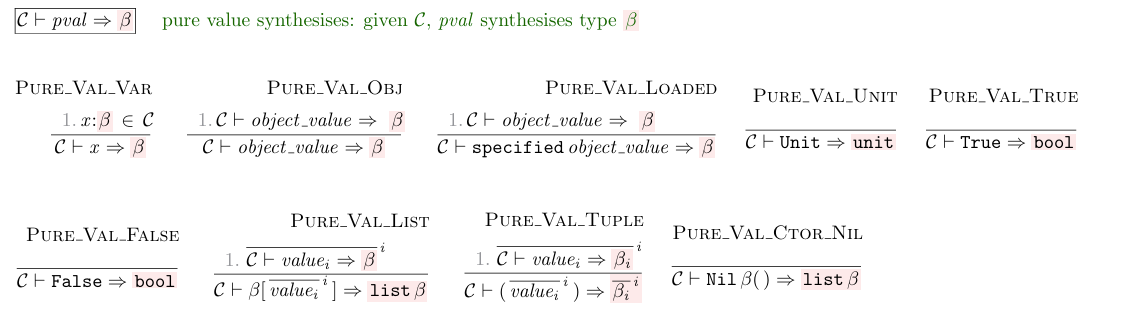
\includegraphics{figures/kernel-pval-typing}
    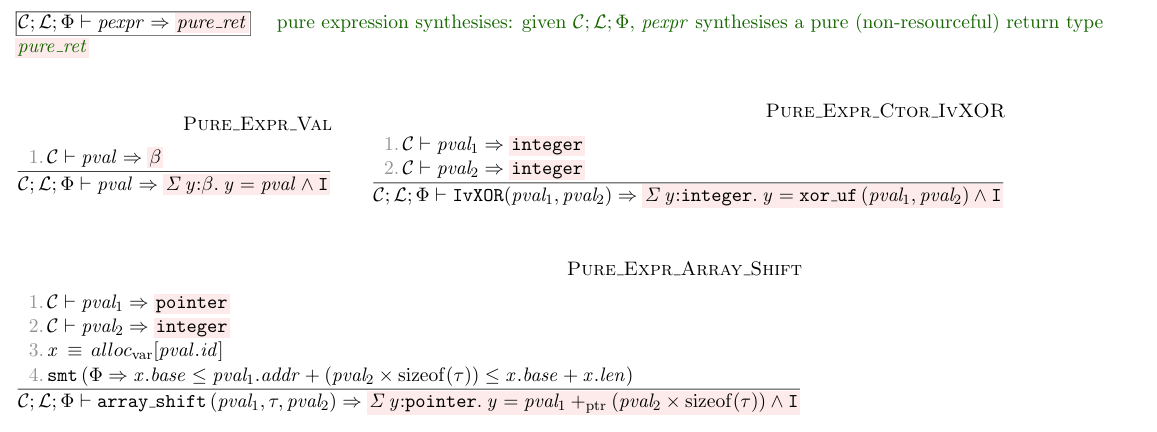
\includegraphics{figures/kernel-pexpr-typing}
    \caption{\kl{Kernel CN} typing rules for pure values and expressions.}\label{fig:typing-pval-pexpr}
\end{figure*}

\section{Top-level pure value values and expressions}


\section{Resource terms}\label{sec:typing-res-terms}

\section{Pattern matching}

\section{Memory actions and operations}

\section{Spine judgement}

\section{Effectful values and expressions}

\section{Top-level effectful values and expressions}

\section{Elaboration}


\subsection{Heap types}\label{subsec:heap-types}

\subsection{Resource Terms, Quantifier Inference}\label{subsec:resq-inf}

Explain \intro{bidirectional} (for quantifiers), linear resources, constraints.
Explicit witness to having permissions, which are linearly typed (just ingredients).
Explain enough rules \textemdash{} typing, operations, especially the weird heaps.
And of course, type safety statement and its proof.
Linear terms in a refinement type system.

(Dep ML, L3, ATS)

Different and unusual compared to Iris style \textemdash{} separation proofs outside the program.

Proof term in one sense, but also factors out operations for resource manipulation.

\subsection{Heaps}


\subsection{Type Safety}


\chapter{Kernel CN:\ Proof of soundness}%
\label{chap:kernel-soundness}

Weird heaps.

\chapter{Informing implementation discussions}\label{chap:inform-impl}

In the early stages, \kl{CN} was implemented by Christopher Pulte and Thomas
Sewell, based on sketches by Neel Krishnaswami. I started formalising
\kl{Kernel CN} much later, and benefited by the clarity of having an
implementations and implementers which and whom I could refer to in moments of
confusion.

However, this mode of development means that there were \emph{many} design
decisions made in a rather conservative context, because the programming was
always of a system which was being defined along the way, rather than a
well-understood pre-existing one. Extensions to syntax and inference were
always the minimum required for verifying the pKVM buddy allocator, lest
performance and inference suffer greatly, rather than ones based on a strong
formal and holistic consideration of the constructs and interactions at play.

As such, there are several restrictions in the implementation, which with the
benefit of hindsight and formalism, are completely unnecessary, but persist as
technical debt. This chapter list a few of these, and explains how the
formalisation brings much needed clarity to many questions around the
implementation.

\url{https://github.com/rems-project/cerberus/labels/language}
\url{https://github.com/rems-project/cerberus/labels/resource\%20reasoning}

\section{Supporting partially initialised reads of structs/unions}

This is not asked for, and actually seems to add a non-trivial amount of noise
and book-keeping to the formalisation. This suggests that the feature is not
worth implementing in CN unless a strong use-case comes up.

\section{Auto unfolding scheme for logical functions}
\url{https://github.com/rems-project/cerberus/issues/483}

\section{Higher-order resources}
\url{https://github.com/rems-project/cerberus/issues/483}

\section{Restrictions on branching}\label{sec:restriction-branching}
\url{https://github.com/rems-project/cerberus/issues/483}
\url{https://github.com/rems-project/cerberus/issues/266}

\section{Removing the pointer first restriction on predicates}\label{sec:rm-ptr-first}
\url{https://github.com/rems-project/cerberus/issues/303}

\section{Unifying the syntax of functions, predicates and specifications}
\url{https://github.com/rems-project/cerberus/issues/304}


\chapter{An alternative presentation}\label{chap:kernel-alternative}

Perhaps a short chapter about MiniCN\@? This could demonstrate the strong
advantages of defining a type system over a first-order functional language,
rather than trying to do so directly over something C-like.

It would also give some space to the interesting but yet-to-be-baked ideas
from the Fuliminate paper.


